\documentclass[12pt]{article}
\usepackage{graphicx}
\usepackage{amsmath}
\usepackage{geometry}
\geometry{vmargin={1in,1in}, hmargin={1in, 1in}}
\usepackage[utf8]{inputenc}
\usepackage{cite}
\usepackage{tabularx,ragged2e,booktabs}
\begin{document}

\title{Article title}
\author{Author's Name}

\maketitle

\begin{abstract}
The abstract .
\end{abstract}

\section{Introduction}Iintroduction.

\section{Model}
Out of all \textit{P. vivax} mathematical models that had been developed in the past, White's model\cite{white2014modelling} is quite interesting as this is the only model that considers variation of hypnozoites in human liver. Models in the past which were deterministic compartmental considered a single compartment to represent humans who developed hypnozoites after recovery. But White's model considered different compartments to represents both susceptible and infected humans according to the number of hypnozoited developed within their liver. 

\begin{figure}[h]
\centering
  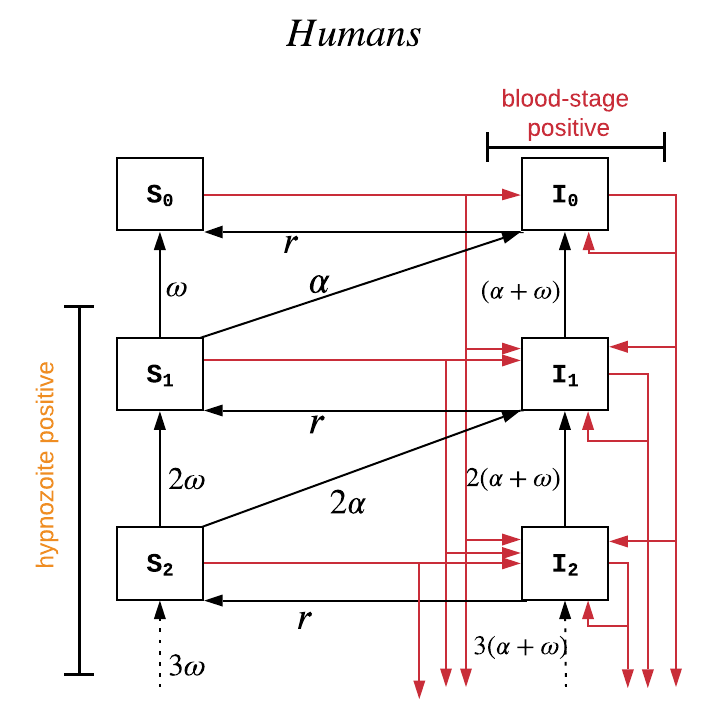
\includegraphics[width=90mm]{White.png}
  \caption{\textit{Schematic representation of the White \textit{et al.} model. $S_i$ represents the fraction of human  population that are susceptible with $i$ hypnozoites and $I_i$ represents the fraction of human population that have  blood-stage infection with $i$ hypnozoites. The mosquito compartment isn't shown here}}
  \label{fig:white}
\end{figure}

Figure \ref{fig:white} shows the model diagram. $S_i$ and $I_i$ represents the fraction of susceptible and infected individuals with $i$ number of hypnozoites respectively. Individuals in all compartments are exposed to primary infections at rate
$\lambda$, following which they will move down the flow
diagram ( shown in red arrow in Figure \ref{fig:white}) to a compartment representing blood-stage
infection and carrying a greater number of hypnozoites. The parameters are described in Table \ref{tab:white}. 




\begin{table}[ht]
\centering
\footnotesize
\caption{Description of the model parameters\label{tab:white}}
\begin{tabular}[t]{cl}
\toprule
\textbf{Symbol} & \textbf{Meaning} \\
\midrule
$a$ & Biting rate of mosquitoes\\
\hline
$b$ & Transmission probability: mosquito to human\\
\hline
$c$ & Transmission probability: human to mosquito\\
\hline
$\omega_m$ & Mosquito death rate\\
\hline
$m$ & Number of mosquitoes per human \\ 
\hline
$n$ & Duration of mosquito sporogony\\
\hline
$r$ & Blood stage infection clearance rate\\
\hline
$\lambda$ & Force of infection\\
\hline
% $N$ & Number of hypnozoites per infection & 8.5 & \cite{white2014modelling} \\
% \hline
$\alpha$ & Hypnozoites activation rate\\
\hline
$\omega $ & Hypnozoite/hepatocyte death rate\\
% $1/\eta$ & duration of prohhylaxis & 7 days & \cite{white2014modelling}\\
% \hline
% $1/\tau$ & time with parasite before clearance by treatment & 14 days & \cite{white2014modelling}\\
% $k_S,k_I$ & treatment coverage & varriy & assumed\\
\bottomrule
\end{tabular}
\end{table}

In White's model, for mosquito dynamics, compartments for susceptible and infected mosquitoes were considered which does not account the incubation period in mosquitoes. In order to consider the delay, we use $S_m$, $E_m$, and $I_m$ to represent fraction of susceptible, exposed, and infected mosquitoes. That is exposed mosquitoes become infected after $n$ days where $n$ is the duration of the incubation period in mosquitoes. We also do not consider superinfection. The equations of the white model are

\begin{align}
    \label{eqn:2.1}
    \frac {dS_i}{dt}=&-\lambda S_i-i(\omega+\alpha)S_i+(i+1)\omega S_{i+1}+rI_i\qquad \qquad i=0,1,2,...\\[12pt]
    \label{eqn:2.2}
    \frac {dI_i}{dt}=&-\lambda I_i+\sum_{j=0}^{i} \lambda_{j\rightarrow i}\left(S_j+I_j\right)-i(\omega+\alpha)I_i+(i+1)(\omega+\alpha)I_{i+1}\notag\\&+(i+1)\alpha S_{i+1}-rI_i\qquad\qquad\qquad\qquad\qquad\qquad  i=0,1,2,...\\[12pt]
    \label{eqn:2.3}
    \frac {dS_m}{dt}=&g-ac\left(\sum_{i=0}^\infty I_i\right)S_m-gS_m,\\[12pt]
    \label{eqn:2.4}
    \frac {dE_m}{dt}=&ac\left(\sum_{i=0}^\infty I_i\right)S_m-(g+\frac{1}{n})E_m, \\[12pt]
    \label{eqn:2.5}
    \frac {dI_m}{dt}=&\frac{1}{n}E_m-gI_m.
\end{align}

where, it is assumed that, the number of hypnozoites following a primary infection is geometrically distributed. That is, if the mean number of hypnozoites established per mosquito bite is $N$, then the probability of $k$ hypnozoites is
\begin{align*}
\lambda_{j\rightarrow i}=&\lambda\left(\frac{N}{N+1}\right)^{i-j}\frac{1}{N+1}.
\end{align*}

Hypnozoites activate at a rate $\alpha$ or die at the rate $\omega$ after a certain period of time. After the activation of death of a hypnozoite, infected individual remain in the infected compartment but now with a less hypnozoites. But in the case of susceptibles, after the activation they move to the infected compartment with a less hypnozoite and in the case of hypnozoite death, they remain in the susceptible compartment with less hypnozoite.  Infected individuals move to the susceptible compartments after the recovery with the same hypnozoites. 

This model is capable of considering infinite number of hypnozoites. This model is a complex one due to the higher number of compartments as well as higher number of differential equation. The idea is to develop a simple model from White's model that captures similar dynamics

We start by setting $S=S_0$, $I=\sum_{i=0}^\infty I_i$, and $H=\sum_{i=1}^\infty S_i$. That is, $S$ represents the fraction of susceptible without any hypnozoites, $I$ represents the fraction of infected individuals and $H$ is fraction of individuals that recovered from the infection with hypnozoites. So we will have only three compartments to represent the dynamics in human population namely SIH. We assume that after recovery, infected individuals who have no hypnozoites developed within will move back to the susceptible compartment with probability $p$ and rest of them move to the H compartment with probability $(1-p)$.

Using this assumption in White's model, we get

\begin{align}
    \label{eqn:2.6}
    \frac {dS}{dt}=&-\lambda S+\omega S_1+prI,\\
    \label{eqn:2.7}
    \frac {dH}{dt}=&-\lambda H-\omega S_1-\alpha(S_1+2S_2+3S_3+\ldots)+(1-p)rI,\\
    \label{eqn:2.8}
    \frac {dI}{dt}=&\lambda(S+H)+\alpha(S_1+2S_2+3S_3+\ldots)-rI.
\end{align}

As $$H=S_1+S_2+S_3+\ldots , $$
we further assume that 
\begin{align*}
    S_1&=k_1H\\
    S_2&=k_2H\\
    S_3&=k_3H\\
    &\ldots\\
    &\ldots
\end{align*}
where $$k_i=\left(\frac{N}{N+1}\right)^{i}\frac{1}{N+1}$$ represents the probability of having $i$ number of hypnozoites within the liver given that the average number is $N$

Then the equations of the SIH model becomes,
\begin{align}
    \label{eqn:2.9}
    \frac {dS}{dt}=&-\lambda S+\omega k_1+prI,\\
    \label{eqn:2.10}
    \frac {dI}{dt}=&\lambda(S+H)+\alpha(k_1+2k_2+3k_3+\ldots)H-rI,\\
    \label{eqn:2.11}
    \frac {dH}{dt}=&-\lambda H-\omega S_1-\alpha(k_1+2k_2+3k_3+\ldots)H+(1-p)rI.
\end{align}



\section{Result}
\section{Discussion}


\section{Conclusion}

\bibliographystyle{acm}
 \bibliography{Ref}

\end{document}